\documentclass[a4paper,11pt]{article}
\input{/home/tof/Documents/Cozy/latex-include/preambule_lua.tex}
\newcommand{\showprof}{show them}  % comment this line if you don't want to see todo environment
\fancyhead[L]{TP jeu de la vie}
\newdate{madate}{10}{09}{2020}
\fancyhead[R]{Première - NSI} %\today
\fancyfoot[L]{~\\Christophe Viroulaud}
\AtEndDocument{\label{lastpage}}
\fancyfoot[C]{\textbf{Page \thepage/\pageref{lastpage}}}
\fancyfoot[R]{\includegraphics[width=2cm,align=t]{/home/tof/Documents/Cozy/latex-include/cc.png}}
\usepackage{tikz}
\begin{document}
\begin{Form}
\begin{commentprof}
Mettre \textbf{mod\_vie.zip} sur le site
\end{commentprof}
\section{Présentation du jeu}
Le jeu de la vie est un automate cellulaire imaginé par John Horton Conway en 1970. C'est un \guill{jeu à zéro joueur}, puisqu'il ne nécessite pas d'intervention. Il se déroule sur une grille à deux dimensions. Les cellules peuvent prendre deux états: \emph{vivantes} ou \emph{mortes}.\\
À chaque étape, l’évolution d’une cellule est entièrement déterminée par l’état de ses huit voisines de la façon suivante:
\begin{itemize}
\item une cellule morte possédant exactement trois voisines vivantes devient vivante (elle naît),
\item une cellule vivante possédant deux ou trois voisines vivantes le reste, sinon elle meurt.
\end{itemize}
Quelques exemples illustrent ces règles simples:
\begin{center}
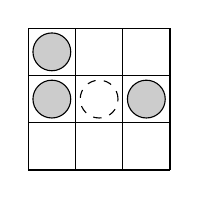
\begin{tikzpicture}[scale=0.6]
\draw (0,0) grid (3,3);
\draw[fill=gray!40](0.5,1.5) circle(0.4);
\draw[fill=gray!40](0.5,2.5) circle(0.4);
\draw[fill=gray!40](2.5,1.5) circle(0.4);
\draw[dashed](1.5,1.5) circle(0.4);
\end{tikzpicture}
\captionof{figure}{Une cellule morte naît car elle a trois voisins}
\end{center}
\begin{center}
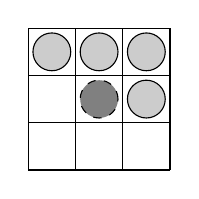
\begin{tikzpicture}[scale=0.6]
\draw (0,0) grid (3,3);
\draw[fill=gray!40](0.5,2.5) circle(0.4);
\draw[fill=gray!40](1.5,2.5) circle(0.4);
\draw[fill=gray!40](2.5,2.5) circle(0.4);
\draw[fill=gray!40](2.5,1.5) circle(0.4);
\draw[fill=gray, dashed](1.5,1.5) circle(0.4);
\end{tikzpicture}
\captionof{figure}{Une cellule vivante meurt car elle a plus de trois voisins}
\end{center}
\begin{center}
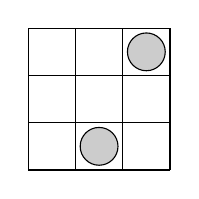
\begin{tikzpicture}[scale=0.6]
\draw (0,0) grid (3,3);
\draw[fill=gray!40](1.5,0.5) circle(0.4);
\draw[fill=gray!40](2.5,2.5) circle(0.4);
\end{tikzpicture}
\captionof{figure}{Une cellule morte le reste car elle n'a que deux voisins.}
\end{center}
\section{Outil graphique}
La bibliothèque \emph{tkinter} est l'interface graphique standard de Python. Le code \ref{base} crée une \emph{fenêtre} graphique et y place un \emph{canevas}. Un canevas est une surface de dessin.
\begin{code}[!h]
\begin{lstlisting}
fenetre = Tk()
fenetre.title("Jeu de la vie")
canevas = Canvas(fenetre, width = 100, height = 100)
canevas.pack()

# ligne à placer en fin de programme
fenetre.mainloop()
\end{lstlisting}
\captionof{code}{Préparer la fenêtre graphique}
\label{base}
\end{code}
\begin{activite}
\begin{enumerate}
\item Créer un fichier jeu-de-la-vie.py et écrire le code \ref{base}.
\item Créer deux variables:
\begin{lstlisting}[xleftmargin=3em,xrightmargin=3em]
TAILLE = 8 #dimension d'une cellule,
CELLULES = 200 #nombre de cellules en largeur et en hauteur.
\end{lstlisting}
Ces deux valeurs seront des constantes du jeu.
\item Modifier le code \ref{base} pour créer un canevas aux bonnes dimensions.
\end{enumerate}
\end{activite}
\section{Préparation du jeu}
\subsection{Créer la grille}
Nous allons représenter les cellules par un tableau de booléens. Chaque ligne contiendra \emph{CELLULES} cases et il y aura \emph{CELLULES} lignes. Une cellule vivante sera codée \emph{True} et une cellule morte, \emph{False}.
\begin{activite}
Construire, en compréhension, le tableau représentant la grille du jeu.
\end{activite}
\subsection{Initialiser la grille}
Pour que le jeu démarre il faut rendre certaines cellules vivantes. Il est possible de les choisir manuellement ou d'en générer aléatoirement un certain nombre.
\begin{activite}
Écrire la fonction \textbf{aleatoire(g: list, n: int)$\;\rightarrow\;$None} qui génère au hasard \emph{n} cellules vivantes dans la grille \emph{g}.
\end{activite}
\subsection{Compter les voisins}
À chaque cycle des cellules naissent ou meurent en fonction de leurs voisins. Pour chaque cellule, il faut donc regarder les huit cellules voisines et compter le nombre de ces cellules qui sont vivantes.
\begin{center}
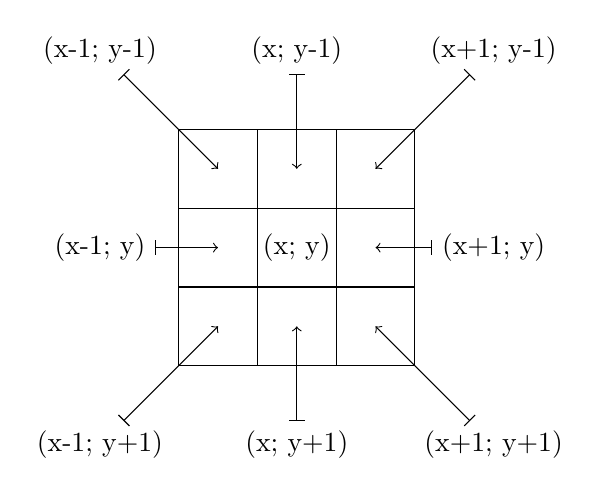
\begin{tikzpicture}
\draw (0,0) grid (3,3);
\node at (1.5,1.5) {(x; y)};

\node (NO) at (-1,4) {(x-1; y-1)};
\node (N) at (1.5,4) {(x; y-1)};
\node (NE) at (4,4) {(x+1; y-1)};
\node (E) at (4,1.5) {(x+1; y)};
\node (SE) at (4,-1) {(x+1; y+1)};
\node (S) at (1.5,-1) {(x; y+1)};
\node (SO) at (-1,-1) {(x-1; y+1)};
\node (O) at (-1,1.5) {(x-1; y)};

\draw[|->] (NO) -- (0.5,2.5);
\draw[|->] (N) -- (1.5,2.5);
\draw[|->] (NE) -- (2.5,2.5);
\draw[|->] (E) -- (2.5,1.5);
\draw[|->] (SE) -- (2.5,0.5);
\draw[|->] (S) -- (1.5,0.5);
\draw[|->] (SO) -- (0.5,0.5);
\draw[|->] (O) -- (0.5,1.5);

\end{tikzpicture}
\captionof{figure}{Coordonnées de cellules voisines\\
}L'axe des ordonnées est orienté vers le bas.
\label{coord}
\end{center}
\begin{activite}
Écrire la fonction \textbf{compter\_voisins(g: list, cel: tuple)$\;\rightarrow\;$int} qui compte et renvoie le nombre de cellules vivantes de la cellule de coordonnées \emph{cel}. Il peut être nécessaire de:
\begin{itemize}
\item utiliser la variable locale \emph{delta},
\begin{lstlisting}[xleftmargin=2em,xrightmargin=1.5em]
delta = ((-1,-1), (-1,0), (-1,1), (0,-1), (0,1), (1,-1), (1,0), (1,1))
\end{lstlisting}
\item penser à gérer les \guill{bords} de la grille.
\end{itemize} 
\end{activite}
\section{Créer le jeu}
\subsection{Réaliser un cycle}
Lors d'un cycle, le jeu regarde chaque cellule de la grille et la fait naître ou mourir en fonction de ses voisines.
\begin{activite}
Compléter la fonction \textbf{cycle (f, c, g: list)$\;\rightarrow\;$None} du code \ref{cycle}. Les paramètres \emph{f, c, g} représentent respectivement la fenêtre tkinter, le canevas et la grille du jeu.
\end{activite}
\begin{code}[!h]
\begin{lstlisting}[xrightmargin=2.5em]
def cycle(f, c, g: list)->None:
    # création d'une nouvelle grille vide
    nouvelle = 

    """
    À RÉALISER
    parcourir la grille g pour faire naître ou mourir les cellules.
    La nouvelle configuration est enregistrée dans la grille 'nouvelle'
    """

    # la grille est actualisée
    g = nouvelle

    # affichage de la grille
    c.delete("all")
    for i in range(CELLULES):
        for j in range(CELLULES):
            if g[i][j]:
            	# création d'un cercle bleu
                c.create_oval(TAILLE*(j),
                                    TAILLE*(i),
                                    TAILLE*(j+1),
                                    TAILLE*(i+1),
                                    fill="blue")
    """    
    nouveau cycle: la méthode after rappelle la fonction
    cycle toutes les 100ms
    """    
    f.after(100, cycle, f, c, g)
\end{lstlisting}
\captionof{code}{La fonction principale du jeu}
\label{cycle}
\end{code}
\subsection{Jouer}
Toutes les fonctions sont maintenant disponibles. Pour jouer, il faut:
\begin{itemize}
\item créer une grille vide,
\item créer une surface tkinter,
\item remplir la grille aléatoirement,
\item lancer le cycle.
\end{itemize}
\begin{activite}
Tester le jeu avec différentes valeurs de cellules initiales.
\end{activite}
\subsection{Des structures prédéfinies}
La bibliothèque \emph{mod\_vie} contient les structures:
\begin{itemize}
\item une\_ligne,
\item aleatoire,
\item vaisseau,
\item canon.
\end{itemize}
\begin{activite}
\begin{enumerate}
\item Télécharger le module sur le site \url{https://cviroulaud.github.io} et le décompresser dans le même dossier que le programme.
\item Importer toutes les fonctions du modules dans le programme.
\item Lancer une fois le programme avec ces nouveaux imports.
\item Dans la console, taper:
\begin{lstlisting}
help(vaisseau)
\end{lstlisting}
Dans Spyder, il est possible de faire apparaître cette aide (la \emph{docstring)} en plaçant le curseur sur la fonction et en appuyant sur les touches \emph{ctrl+i}.
\item Ouvrir le fichier \emph{mod\_vie.py} et observer la construction des docstrings.
\item Utiliser les différentes structures dans le programme.
\end{enumerate}
\end{activite}
Il existe des structures encore plus surprenantes. La vidéo ci-après présente des possibilités incroyables.
\begin{center}
\url{https://tinyurl.com/ybhy4n3c}
\end{center}
\end{Form}
\end{document}